\documentclass[convert={outfile=\jobname.svg}]{standalone}
\usepackage{tikz}
\usepackage{fontspec}
\setmainfont{Gentium Plus}
\usetikzlibrary{calc}
\usepackage{calc}
\newcommand\DrawControl[3]{
  \node[draw=#3!80,circle,inner sep=2pt,label={left:(#1, #2)}] at ($(0.01 * #1, 0.01 * #2)$) {};
}
\newcommand\DrawPoint[3]{
  \node[thick,circle,fill=#3,inner sep=2pt,label={left:(#1, #2)}] at ($(0.01 * #1, 0.01 * #2)$) {};
}

\pagestyle{empty}
\begin{document}
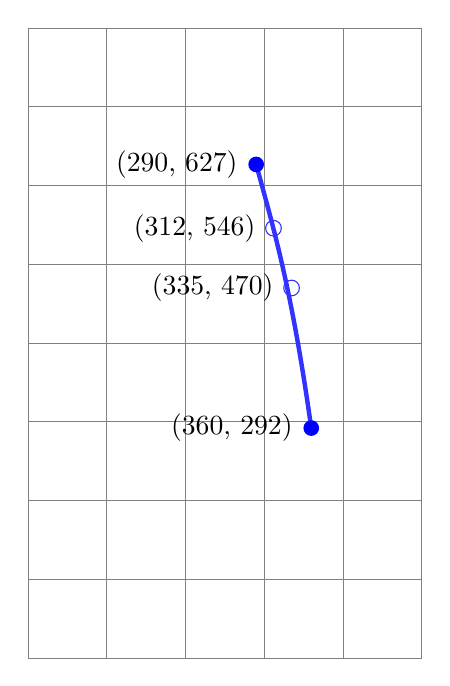
\begin{tikzpicture}
\draw[help lines] (0,0) grid (5,8);
\draw[ultra thick,blue,draw=blue!80]
  (290 * 0.01,627 * 0.01)
    .. controls (312 * 0.01, 546*0.01) and (335 * 0.01, 470 * 0.01) ..
  (360 * 0.01, 292 * 0.01);
  \DrawPoint{360}{292}{blue}
  \DrawControl{312}{546}{blue}
  \DrawControl{335}{470}{blue}
  \DrawPoint{290}{627}{blue}
\end{tikzpicture}\qquad
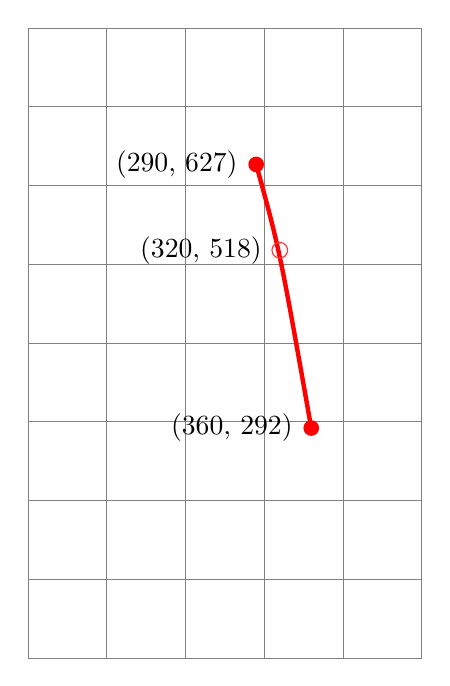
\begin{tikzpicture}
\draw[help lines] (0,0) grid (5,8);
\draw[ultra thick,red]
  (360 * 0.01,292 * 0.01)
    .. controls (320 * 0.01, 518*0.01) ..
  (290 * 0.01, 627 * 0.01);
  \DrawPoint{360}{292}{red}
  \DrawControl{320}{518}{red}
  \DrawPoint{290}{627}{red}
\end{tikzpicture}
\end{document}
